%%%%%%%%%%%%%%%%%%%% author.tex %%%%%%%%%%%%%%%%%%%%%%%%%%%%%%%%%%%
%
% sample root file for your "contribution" to a contributed volume
%
% Use this file as a template for your own input.
%
%%%%%%%%%%%%%%%% Springer %%%%%%%%%%%%%%%%%%%%%%%%%%%%%%%%%%


% RECOMMENDED %%%%%%%%%%%%%%%%%%%%%%%%%%%%%%%%%%%%%%%%%%%%%%%%%%%
\documentclass[graybox]{svmult}

% choose options for [] as required from the list
% in the Reference Guide

\usepackage{type1cm}        % activate if the above 3 fonts are
                            % not available on your system
%
\usepackage{makeidx}         % allows index generation
\usepackage{graphicx}        % standard LaTeX graphics tool
                             % when including figure files
\usepackage{multicol}        % used for the two-column index
\usepackage[bottom]{footmisc}% places footnotes at page bottom


\usepackage{newtxtext}       % 
\usepackage{newtxmath}       % selects Times Roman as basic font

% see the list of further useful packages
% in the Reference Guide

\makeindex             % used for the subject index
                       % please use the style svind.ist with
                       % your makeindex program

%%%%%%%%%%%%%%%%%%%%%%%%%%%%%%%%%%%%%%%%%%%%%%%%%%%%%%%%%%%%%%%%%%%%%%%%%%%%%%%%%%%%%%%%%

\DeclareUnicodeCharacter{2212}{-}
\DeclareUnicodeCharacter{22C5}{-}

\begin{document}

\title*{Recovering from population extinction in the Animal Life Cycle Algorithm (ALCA)} 
\titlerunning{Animal Life Cycle Algorithm (ALCA)}
% Use \titlerunning{Short Title} for an abbreviated version of
% your contribution title if the original one is too long
\author{J. C. Felix-Saul, Mario García Valdez}
% Use \authorrunning{Short Title} for an abbreviated version of
% your contribution title if the original one is too long
\institute{J. C. Felix-Saul \at Tijuana Institute of Technology, Tijuana, Mexico, \email{name@email.address}
\and Mario García Valdez \at Tijuana Institute of Technology, Tijuana, Mexico, \email{name@email.address}}
%
% Use the package "url.sty" to avoid
% problems with special characters
% used in your e-mail or web address
%
\maketitle

\abstract*{In previous work, we introduced an algorithm inspired by the
biological Life Cycle of animal species, consisting of the stages: birth,
growth, reproduction, and death. As in nature, population individuals grow
older and age. In this algorithm's reproduction process, couples must match by
mutual attraction, where sometimes individuals won't procreate offspring
because of the mate's low appeal. As time passes, the environment kills its
individuals either because of low fitness or age, causing occasional population
extinction. When this condition presents, it is required to create a new
population if evaluations are available and termination conditions are
favorable to continue. Some alternatives we explored to restart this new
population are the random generation of a new set of candidate solutions and
the creation of a new set of candidate solutions based on either: a mix of
elements from the best historically found candidate solutions set (Elite); the
mutation with uniform modification from the Elite or the historically
best-found solution (Champion); crossing the Champion with the Elite; the
projection of the Elite towards the Champion; based on random use of the
previous alternatives. In this paper, we present one of the most promising
alternatives to solve population extinction caused by nature's pressure in the
Life Cycle algorithm: the projection of the Elite towards the Champion, where
we compare the results obtained with the latter and the random use of all the
alternatives, using classic benchmark functions for optimization for
comparison.}

\abstract{In previous work, we introduced an algorithm inspired by the
biological Life Cycle of animal species, consisting of the stages: birth,
growth, reproduction, and death. As in nature, population individuals grow
older and age. In this algorithm's reproduction process, couples must match by
mutual attraction, where sometimes individuals won't procreate offspring
because of the mate's low appeal. As time passes, the environment kills its
individuals either because of low fitness or age, causing occasional population
extinction. When this condition presents, it is required to create a new
population if evaluations are available and termination conditions are
favorable to continue. Some alternatives we explored to restart this new
population are the random generation of a new set of candidate solutions and
the creation of a new set of candidate solutions based on either: a mix of
elements from the best historically found candidate solutions set (Elite); the
mutation with uniform modification from the Elite or the historically
best-found solution (Champion); crossing the Champion with the Elite; the
projection of the Elite towards the Champion; based on random use of the
previous alternatives. In this paper, we present one of the most promising
alternatives to solve population extinction caused by nature's pressure in the
Life Cycle algorithm: the projection of the Elite towards the Champion, where
we compare the results obtained with the latter and the random use of all the
alternatives, using classic benchmark functions for optimization for
comparison.}

%\keywords{Distributed Bioinspired Algorithms \and Genetic Algorithms \and Cloud Computing.}

\newpage
\section{Introduction}
\label{sec:1}

Bio-inspired algorithms have been very successful when used to solve complex
optimization problems
\cite{castillo2019comparative,valdez2021swarm,acherjee2020ultrasonic}, but as
their complexity increases so does the computing power required
\cite{ontiveros2018high}. One strategy to address this processing need is to
use distributed computing \cite{thain2005distributed}, or the resources
available in the cloud \cite{garcia2013there,eshratifar2019bottlenet} to help
find the solution. This strategy gives us elasticity to adjust (increase or
reduce) the computing power to achieve a balance according to the nature of the
problem.

One of the problems that we have identified in this research is that most
bio-inspired algorithms are designed with a traditionally sequential
perspective \cite{porto2018evolutionary,back1996evolutionary}, where each
process must wait for the previous task to finish before continuing. Some
architectures address this issue
\cite{valdez2021container,garcia2015evospace,merelo2016nodio}, what
distinguishes this proposal is the introduction of  an algorithm designed in its
entirety as a native solution in the cloud, fully distributed, where its
processes are executed in parallel and interaction takes place asynchronously. This technique makes it
easy to scale the computing power according to the complexity required by the
problem \cite{armbrust2010view}.

We designed our algorithm using observation, analysis, and abstraction in
nature to identify what most species in the animal kingdom have in common,
where individuals of a population that best adapt to the environment have
greater chances of survival, reproduction, and improvement of the species.
Imagining as if the task of writing these rules of evolution was in our hands,
questioning how we could solve it?

Like nature, we identified what most species have in common in the life cycle.
Our algorithm works on a constantly evolving population, experiencing the
stages that all living beings undergo \cite{read1968system}: being born,
growing up, reproducing, and dying, where each of these stages will be
processes (of our algorithm) that randomly affect the population individuals,
emulating the organic way.

The main contribution of the paper is to design and create a new algorithm with
the purpose to demonstrate that it is possible to evolve a population of
individuals, similar to a Genetic Algorithm (GA), using a distributed,
parallel, and asynchronous methodology by implementation and testing of the
algorithm. 

We present the description of the following sections in our paper. First, we
introduce our algorithm inspired by the Life-Cycle of animal species in
% Please use capitalization consistently; I don't think this should go in Caps - JJ
section~\ref{section.proposal}, followed by our experimental configuration and
results in section~\ref{section.experiments}, we analyze and describe some of
our research findings in section~\ref{section.discussion}, and we finalize by
presenting some inferences based on our experiments' results in
section~\ref{section.conclusions}.


\section{Proposal}
\label{section.proposal}
% Always give a unique label
% and use \ref{<label>} for cross-references
% and \cite{<label>} for bibliographic references
% use \sectionmark{}
% to alter or adjust the section heading in the running head

Many of the publications with the most influence on our research
~\cite{valdez2021container,garcia2021event,merelo2016performance,merelo2016nodio}
propose a cloud-native optimization architecture that features population-based
algorithms. They present ideas such as those mentioned in Figure~\ref{fig.background},
which planted the seed of thought of our current paper.

\begin{figure}
    \centering
    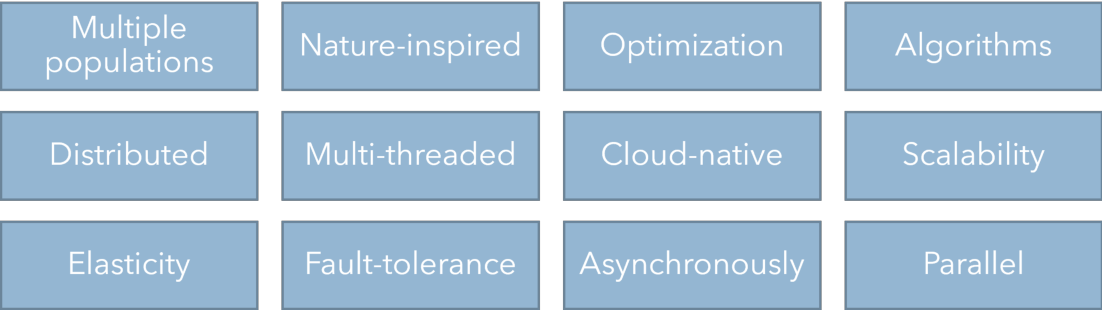
\includegraphics[width=80mm]{img/fig1_background.pdf}
    \caption{These ideas planted the seed of thought in our algorithm proposal.} \label{fig.background}
    \end{figure}

Our main inspiration for this algorithm was born from the study and observation
of nature, where many successful optimization algorithms have previously found
their own. Our focus was not on a single animal species but all of them, using
general abstraction to identify what those species have in common. 

Some questions in our train of thought were: How does nature work? Is evolution
real? How do we enforce natural selection in evolution? What is the role of the
attraction between couples on reproduction? How much of a factor is the
attraction's role in the evolution of the species? What is the role of death in
all of this? How much of an impact does death have on the evolution of a
species? How do we include those ideas into our algorithm?

In our analysis, we consider a broad animal spectrum, from bacteria to humans
and lions, finding our inspiration on the biological Life Cycle of the animal
species, which consists of several stages \cite{read1968system}: birth, growth,
reproduction, and death. As in nature, we intend to execute all these stages in
parallel and asynchronously on a population that evolves constantly. The
combination of those processes is what we call evolution.

One of the main challenges when designing the algorithm was how to capture the
essence of life by reflecting a population evolution?. In our minds, it was
clear this task requires a combination of simultaneous working forces that
influences the population improvement over time. Our strategy was simple:
divide and conquer, looking into the clouds. Enter cloud-computing: previous
cloud-computing algorithms have proven successful results working in
optimization problems \cite{valdez2021container,garcia2021event}.

We turned back to our genetic algorithms knowledge, mixed with our inspiration
and cloud computing, and designed the algorithm with the quest to divide the
processing workload among multiple computers. This strategy would also make it
possible to run our algorithm as a cloud service. Theoretically, one
consequence of the workload distribution is to obtain lower execution times.

This algorithm seeks to imitate the natural life cycle, where new individuals
are born at any moment and mature over time, where they age and suffer
mutations throughout their lives. In reproduction, couples match by mutual
attraction, and they may have offspring. Death can happen to everyone: from a
newborn to an aged adult, where the individual's fitness will impact their
longevity. The general model concept is shown in Figure~\ref{fig.proposal}. The general
flowchart for the Life-Cycle algorithm is described in Figure~\ref{fig.flowchart}.

\begin{figure}
    \centering
    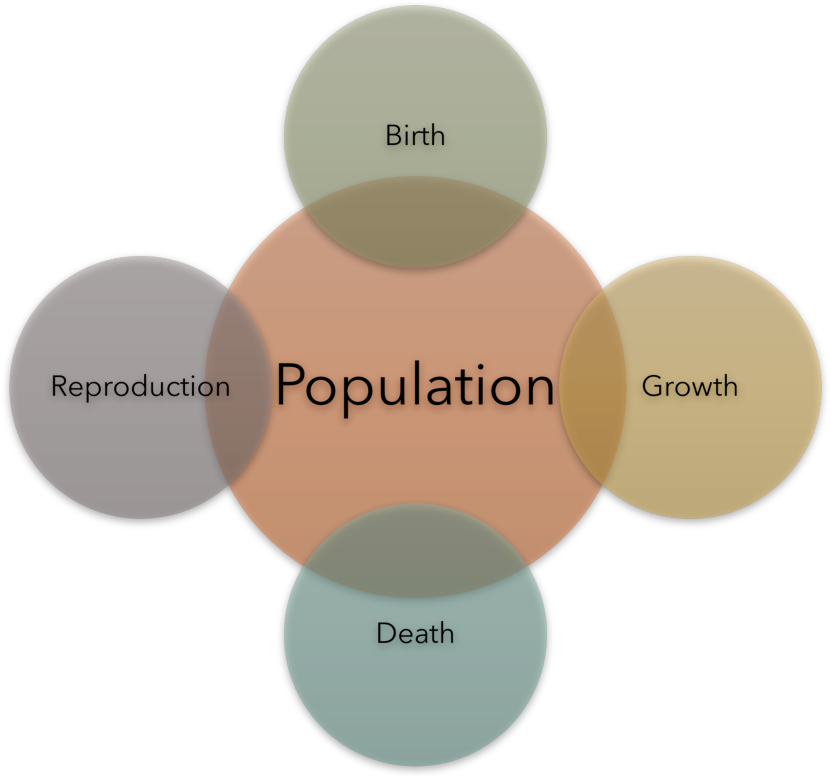
\includegraphics[width=70mm]{img/fig2_proposal.pdf}
    \caption{Algorithm model inspired by the animal species' biological Life-Cycle.} \label{fig.proposal}
    \end{figure}

\begin{figure}
    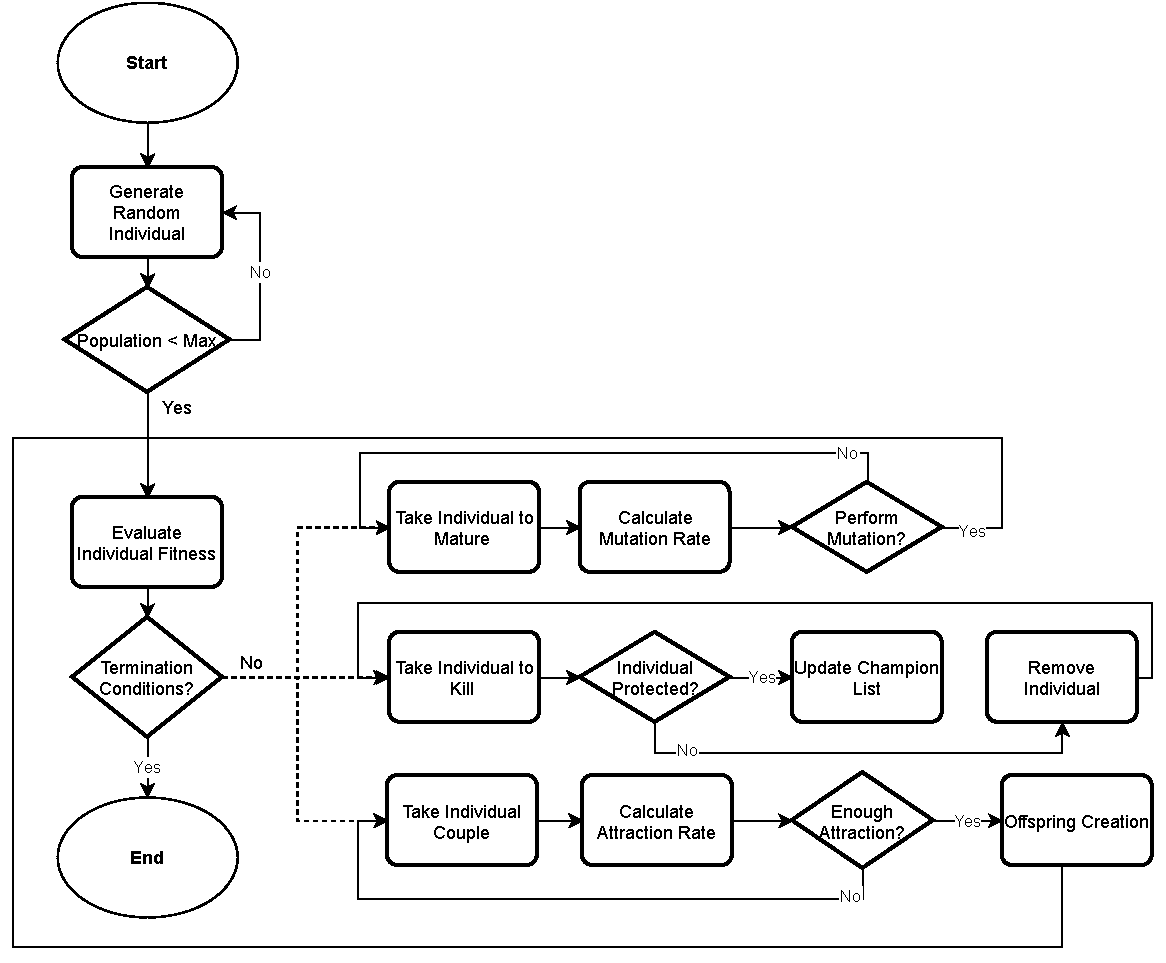
\includegraphics[width=\textwidth]{img/fig4_flowchart.pdf}
    \caption{Life-Cycle algorithm general flowchart.} \label{fig.flowchart}
% Several terms are introduced here that are not defined in the text, like "champion list" and "attraction" - JJ
    \end{figure}
    

\subsection{Birth}

This algorithm starts with a randomly generated population, where the processes
will interact with the population independently. This means that at any given
time, any individual can experience any of these processes. Birth is the first
process of our algorithm, and it is responsible for the initial generation of
individuals.

\subsection{Growth}

As in nature, all individuals constantly grow, mature, or age. With increasing
age, individuals may lose strength but also gain more knowledge to solve
problems. We represent this with a possible mutation in each increment of age.
The growth process will take an individual to assess whether it's ready to
mature and undergo changes. % Not learning?  JJ

\subsection{Reproduction}

The attraction of a couple will depend on fitness: the better individual's
fitness, the more attractive it will be, making it easier to find mating
matches. This process will be taking random pairs of individuals to evaluate
their attraction as a couple, to try to breed; when the gestation is
successful, a new pair of individuals will be born (as the offspring). Not all
couples will be compatible, so reproduction will not always be possible, but
the problem arises: how to quantify the attraction between two individuals?

We could have used several strategies to evaluate this attraction. Considering
this algorithm takes a similar focus as the study of bacteria growth in
microbiology, where we can observe and analyze the evolution of a population
over time. As in nature' most species, the bigger a specimen is, the more
attractive it is to its mating candidates. To be consistent with both ideas in
% Er... not really. It depends on health, mainly - JJ
our algorithm, we use the equation of Newton's Law of Universal Gravitation (1)
to calculate the attraction between two individuals, where we visualize the
individual fitness as its mass when using the equation. In previous work,
Newton's Law of Universal Gravitation has shown success in helping to solve
optimization problems \cite{sanchez2014fuzzy,rashedi2009gsa}.

\begin{figure}
    \centering
    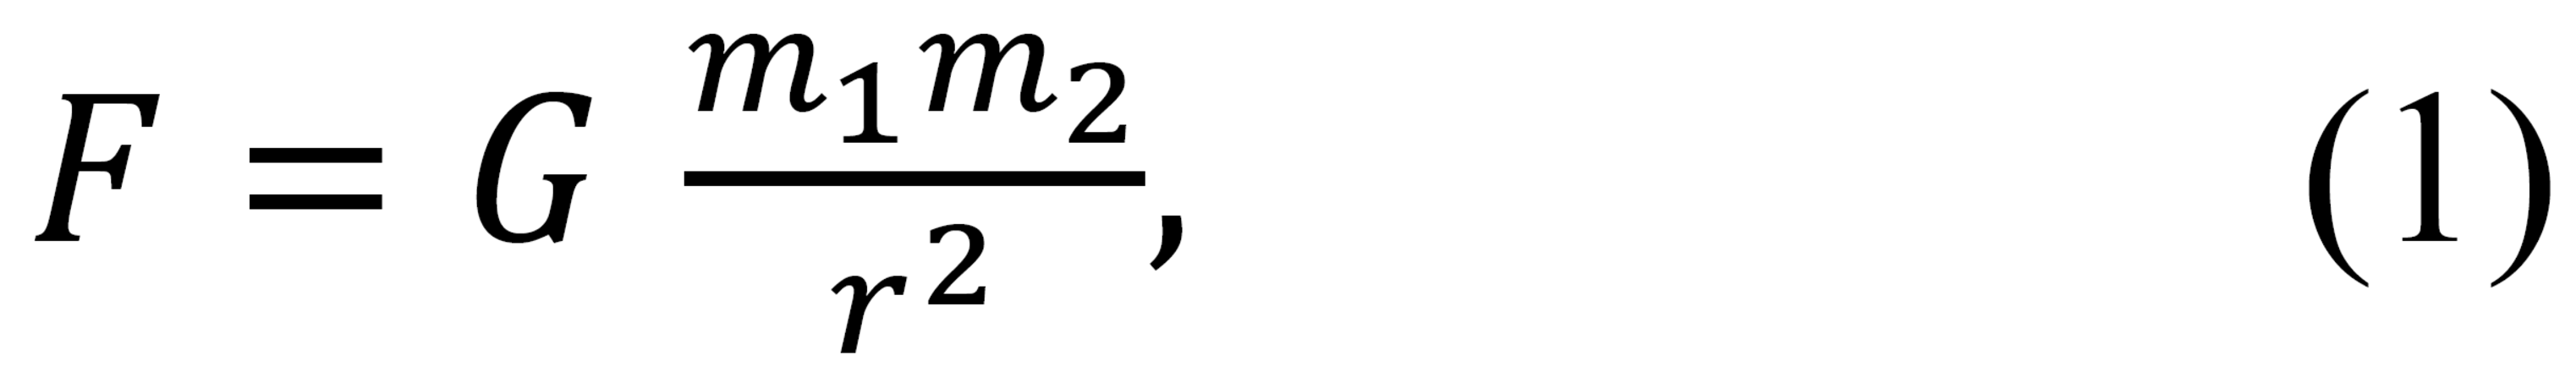
\includegraphics[width=50mm]{img/fig3_newtonslaw.pdf}
    \caption{Newton's Law of Universal Gravitation.} \label{fig.newtonslaw}
    \end{figure}

Where:
\begin{itemize}
    \item[]	    F is the gravitational force acting between two objects.
    \item[]	    m1 and m2 are the masses of the objects.
    \item[]	    r is the distance between the centers of their masses.
    \item[]	    G is the gravitational constant: 6.67430(15)×10−11 m3⋅kg−1⋅s−2.
\end{itemize}

% to be honest, I find this a bit far fetched. How do you define mass? is it related to fitness? - JJ

\subsection{Death}

The death stage represents the challenges and adversities that life presents to
overcome. This process evaluates the individual resistance to survive in the
environment. The better fitness the individual has will increase its chances of
survival. As time progresses, the demands of nature will also increase, pushing
for only the best individuals to survive.


\section{Experiments}
\label{section.experiments}

As a proof-of-concept, we implemented the algorithm with Docker containers by
solving the OneMax problem to compare it with a traditional GA algorithm using
the DEAP (Distributed Evolutionary Algorithms in Python) library
\cite{fortin2012deap}. The OneMax problem \cite{krejca2020lower,witt2019upper}
uses a genetic algorithm to evolve a population of randomly generated
individuals with zeros and ones, and it stops until a solution of only ones is
found.

\subsection{Experimental Setup}

\begin{figure}
    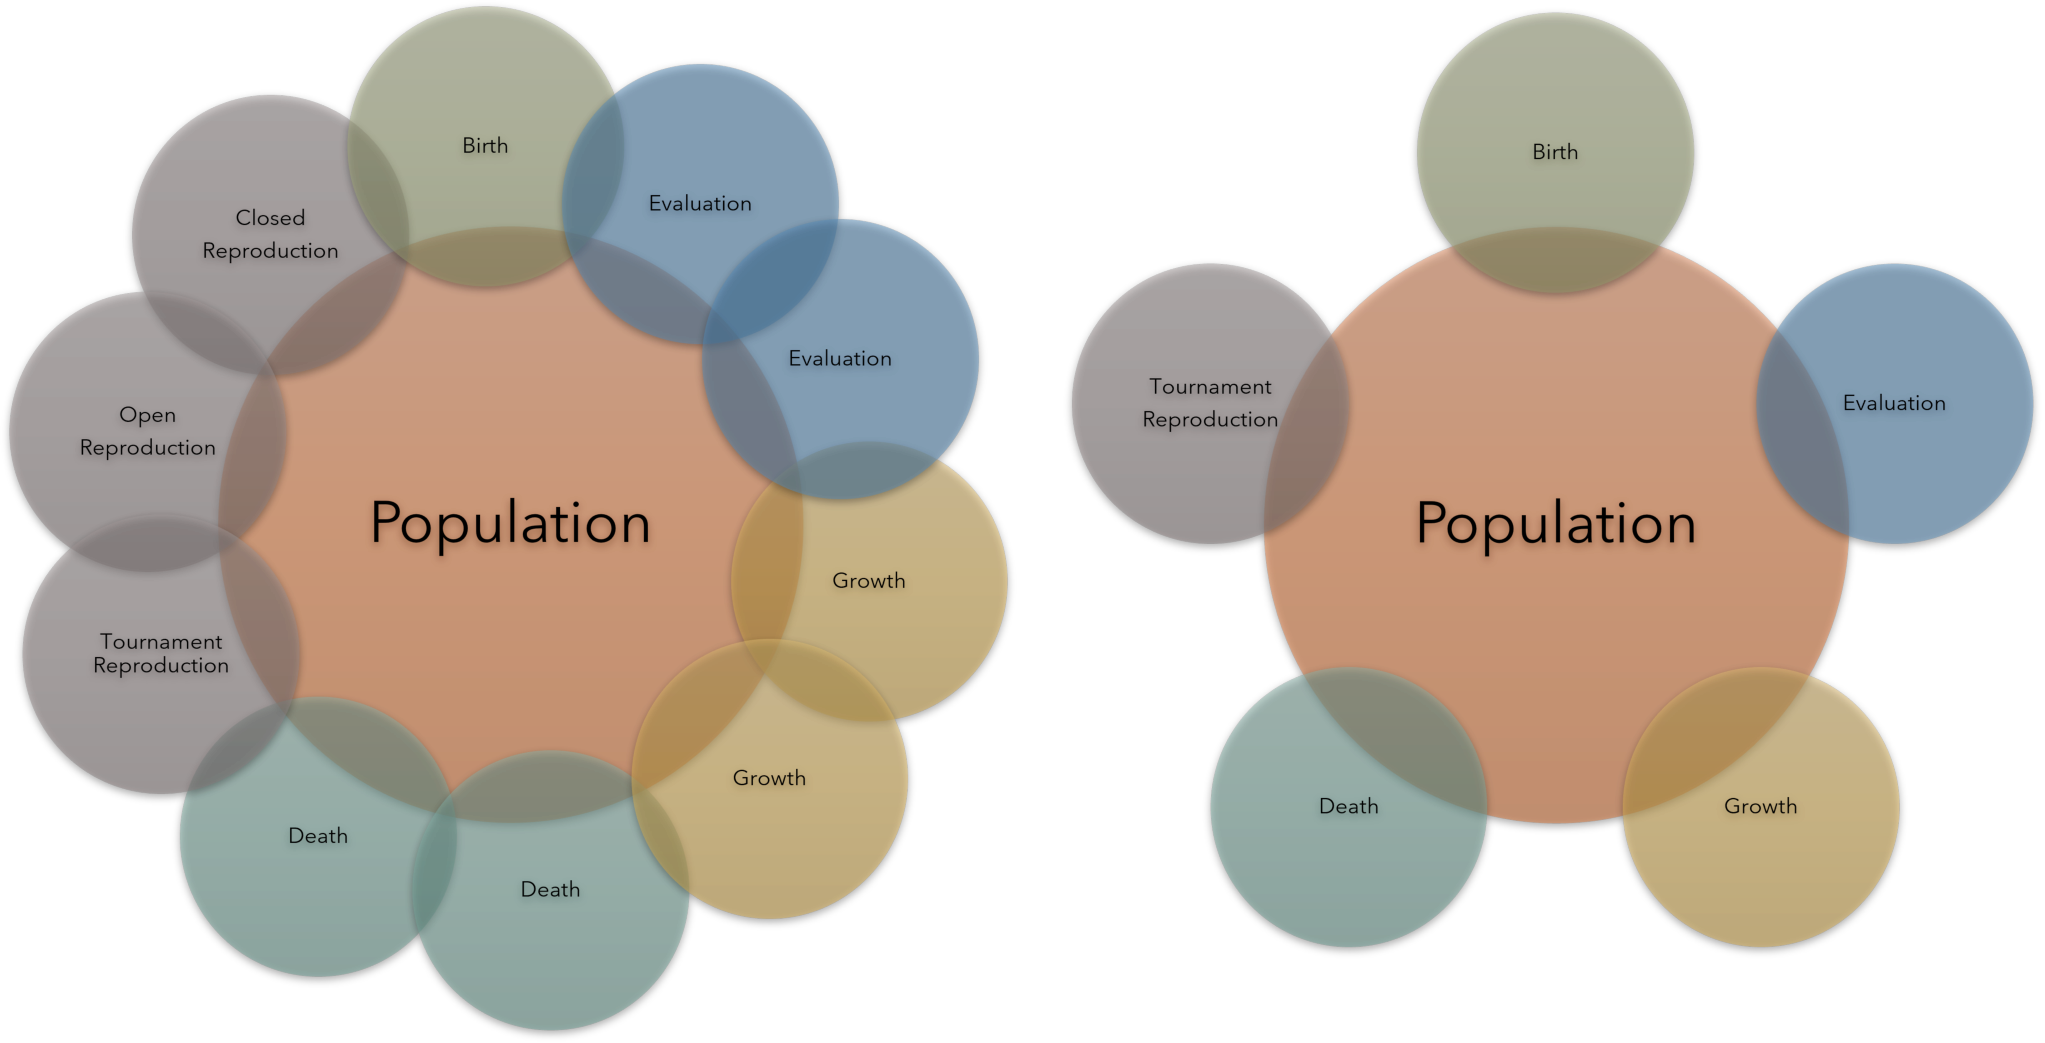
\includegraphics[width=\textwidth]{img/fig5_processes_containers.pdf}
    \caption{Life-Cycle algorithm processes in containers comparison.} \label{fig.processes_containers}
    \end{figure}

One strategic difference in our algorithm implementation is the reproduction
process, which is flexible to work in parallel with multiple couple selection
methods, for example, tournament selection, random selection (Closed
Reproduction process), and couple match by creating a new mating individual
(Open Reproduction process). We use many combinations of the containerized
processes, up to the minimum number required to obtain good results.
Figure~\ref{fig.processes_containers} shows a comparison of only two alternatives for the
implementation of the algorithm. Our experimentation started with a
configuration of ten processes and ended in five, shown on the left and right
sides of Fig.~\ref{fig.processes_containers}, respectively.

\subsection{Experiment Configuration}

In our four experiments, we needed to match or balance the experimentation
parameters according to the specifications of the algorithm used by the DEAP
library. This is to be able to verify if our algorithm would also converge on
the solutions in a similar number of evaluations and execution time.
Table~\ref{tab.configuration} shows the OneMax initial configuration for DEAP and Life-Cycle
experiment.

\begin{table}[]
    \centering        
    \caption{OneMax initial configuration for DEAP and Life-Cycle experiment.}\label{tab.configuration}
    \begin{tabular}{|l|l|l|}
    \hline
    \textbf{Configuration} & \textbf{DEAP} & \textbf{Life-Cycle} \\ \hline
    Population & 60 & 60 \\ \hline
    Max Generation & 20 & 20 \\ \hline
    Stagnation & Off & 10 \\ \hline
    Chromosome Length & 20 & 20 \\ \hline
    Target Fitness & 20 & 20 \\ \hline
    Crossover Rate & 100 & 100 \\ \hline
    Mutation Rate & 7 & 7 \\ \hline
    Tournament Rate & 100 & 50 \\ \hline
    Tournament Sample & 3 & 4 \\ \hline
    Open Reproduction Rate & NA & 5 \\ \hline
    Closed Reproduction Rate & NA & 45 \\ \hline
    Max Age & NA & 80 \\ \hline
    Base Approval & NA & 80 \\ \hline
    Goal Approval & NA & 100 \\ \hline
    \end{tabular}
    \end{table}


\subsection{Experiment Results}

For each experiment, we ran 60 independent executions per algorithm and
recorded the following results: Last Generation, Total Evaluations, Time
(seconds), Evaluations/second. The labels used on the results of our summarized
experiments tables are the following:

\begin{itemize}
    \item   Last Gen.   is the generation that found the solution.
    \item   Eval.       is the total number of evaluations the algorithm executed. 
    \item   Time (sec)  is the total elapsed or wall clock time, in seconds. 
    \item   Eval/sec    is the calculated rate of evaluations per second.
\end{itemize}


\subsubsection{Experiment 1} The goal of our first OneMax experiment was to
make sure our Life-Cycle algorithm worked as expected, converging on the
solution. For this experiment, we intentionally used delays (on the tenth of a
second magnitude) to follow the Life-Cycle algorithm behavior on the console
output. For this experiment, we compared the DEAP algorithm versus the
Life-Cycle using ten processes (on containers) where we show the summarized
results in Table~\ref{tab.experiment1}, and Figure~\ref{fig.experiment1} shows
their Box and Whisker chart.

\begin{table}[]
    \centering        
    \caption{Experiment 1 results: OneMax DEAP versus Life-Cycle (10 processes).}\label{tab.experiment1}
    \begin{tabular}{|l|l|l|l|l|l|l|l|l|}
    \hline
    Run & \multicolumn{4}{l|}{OneMax DEAP} & \multicolumn{4}{l|}{Life-Cycle (10P)} \\ \hline
    1-60 & Last Gen. & Eval. & Time (sec) & Eval/sec & Last Gen. & Eval. & Time (sec) & Eval/sec \\ \hline
    Avg. & 6.5 & 391 & 0.036 & 10,836 & 9.6 & 578 & 6.830 & 85 \\ \hline
    \end{tabular}
    \end{table}

\begin{figure}
    \fbox{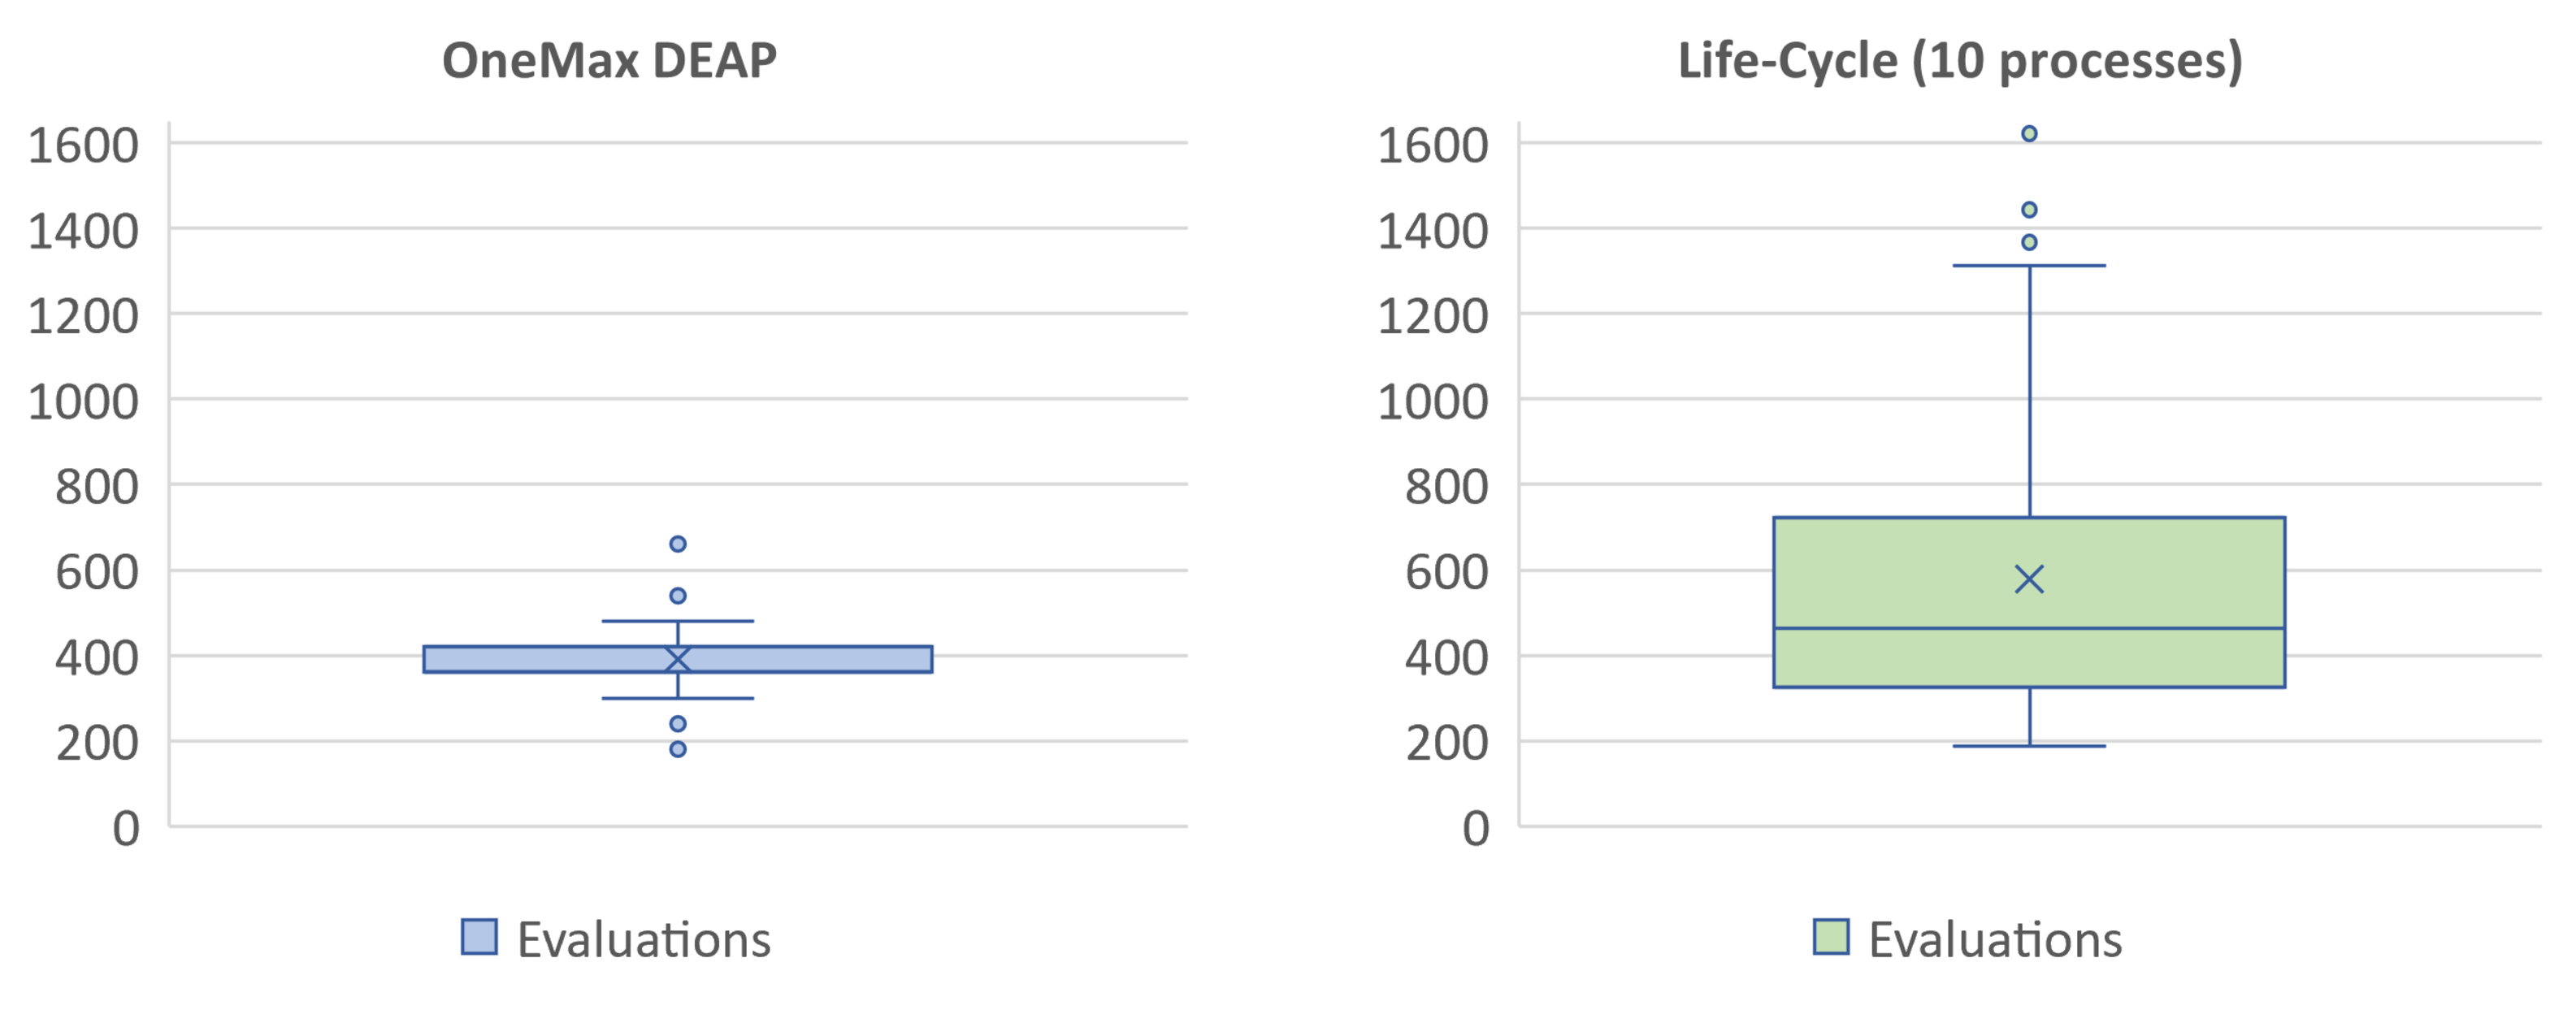
\includegraphics[width=\textwidth]{img/fig6_experiment01_chart.pdf}}
    \caption{Box and whisker chart for the Experiment 1: OneMax DEAP versus Life-Cycle.} \label{fig.experiment1}
% You need to label axis y - JJ
  \end{figure}


\subsubsection{Experiment 2} The goal of our second experiment was to confirm
the Life-Cycle algorithm continued working as expected, converging on the
solution. For this experiment, we reduced the time used on delays (now on the
thousands of a second magnitude) to follow the Life-Cycle algorithm behavior.
For this experiment, we only used tournament selection for the reproduction, on
the first configuration running the Life-Cycle on ten processes, versus the
second configuration where we reduced the processes to the minimum basic 5. We
show the summarized results in Table~\ref{tab.experiment2}, and
Figure~\ref{fig.experiment2} shows their Box and Whisker chart.

\begin{table}[]
    \centering        
    \caption{Experiment 2 results, Life-Cycle Tournament selection: 10 versus 5 processes.}\label{tab.experiment2}
    \begin{tabular}{|l|l|l|l|l|l|l|l|l|}
    \hline
    Run & \multicolumn{4}{l|}{LifeCycle (Tourn. 10P)} & \multicolumn{4}{l|}{LifeCycle (Tourn. 5P)} \\ \hline
    1-60 & Last Gen. & Eval. & Time (sec) & Eval/sec & Last Gen. & Eval. & Time (sec) & Eval/sec \\ \hline
    Avg. & 7.2 & 434 & 0.740 & 587 & 8.2 & 495 & 0.826 & 599 \\ \hline
    \end{tabular}
    \end{table}

\begin{figure}
    \fbox{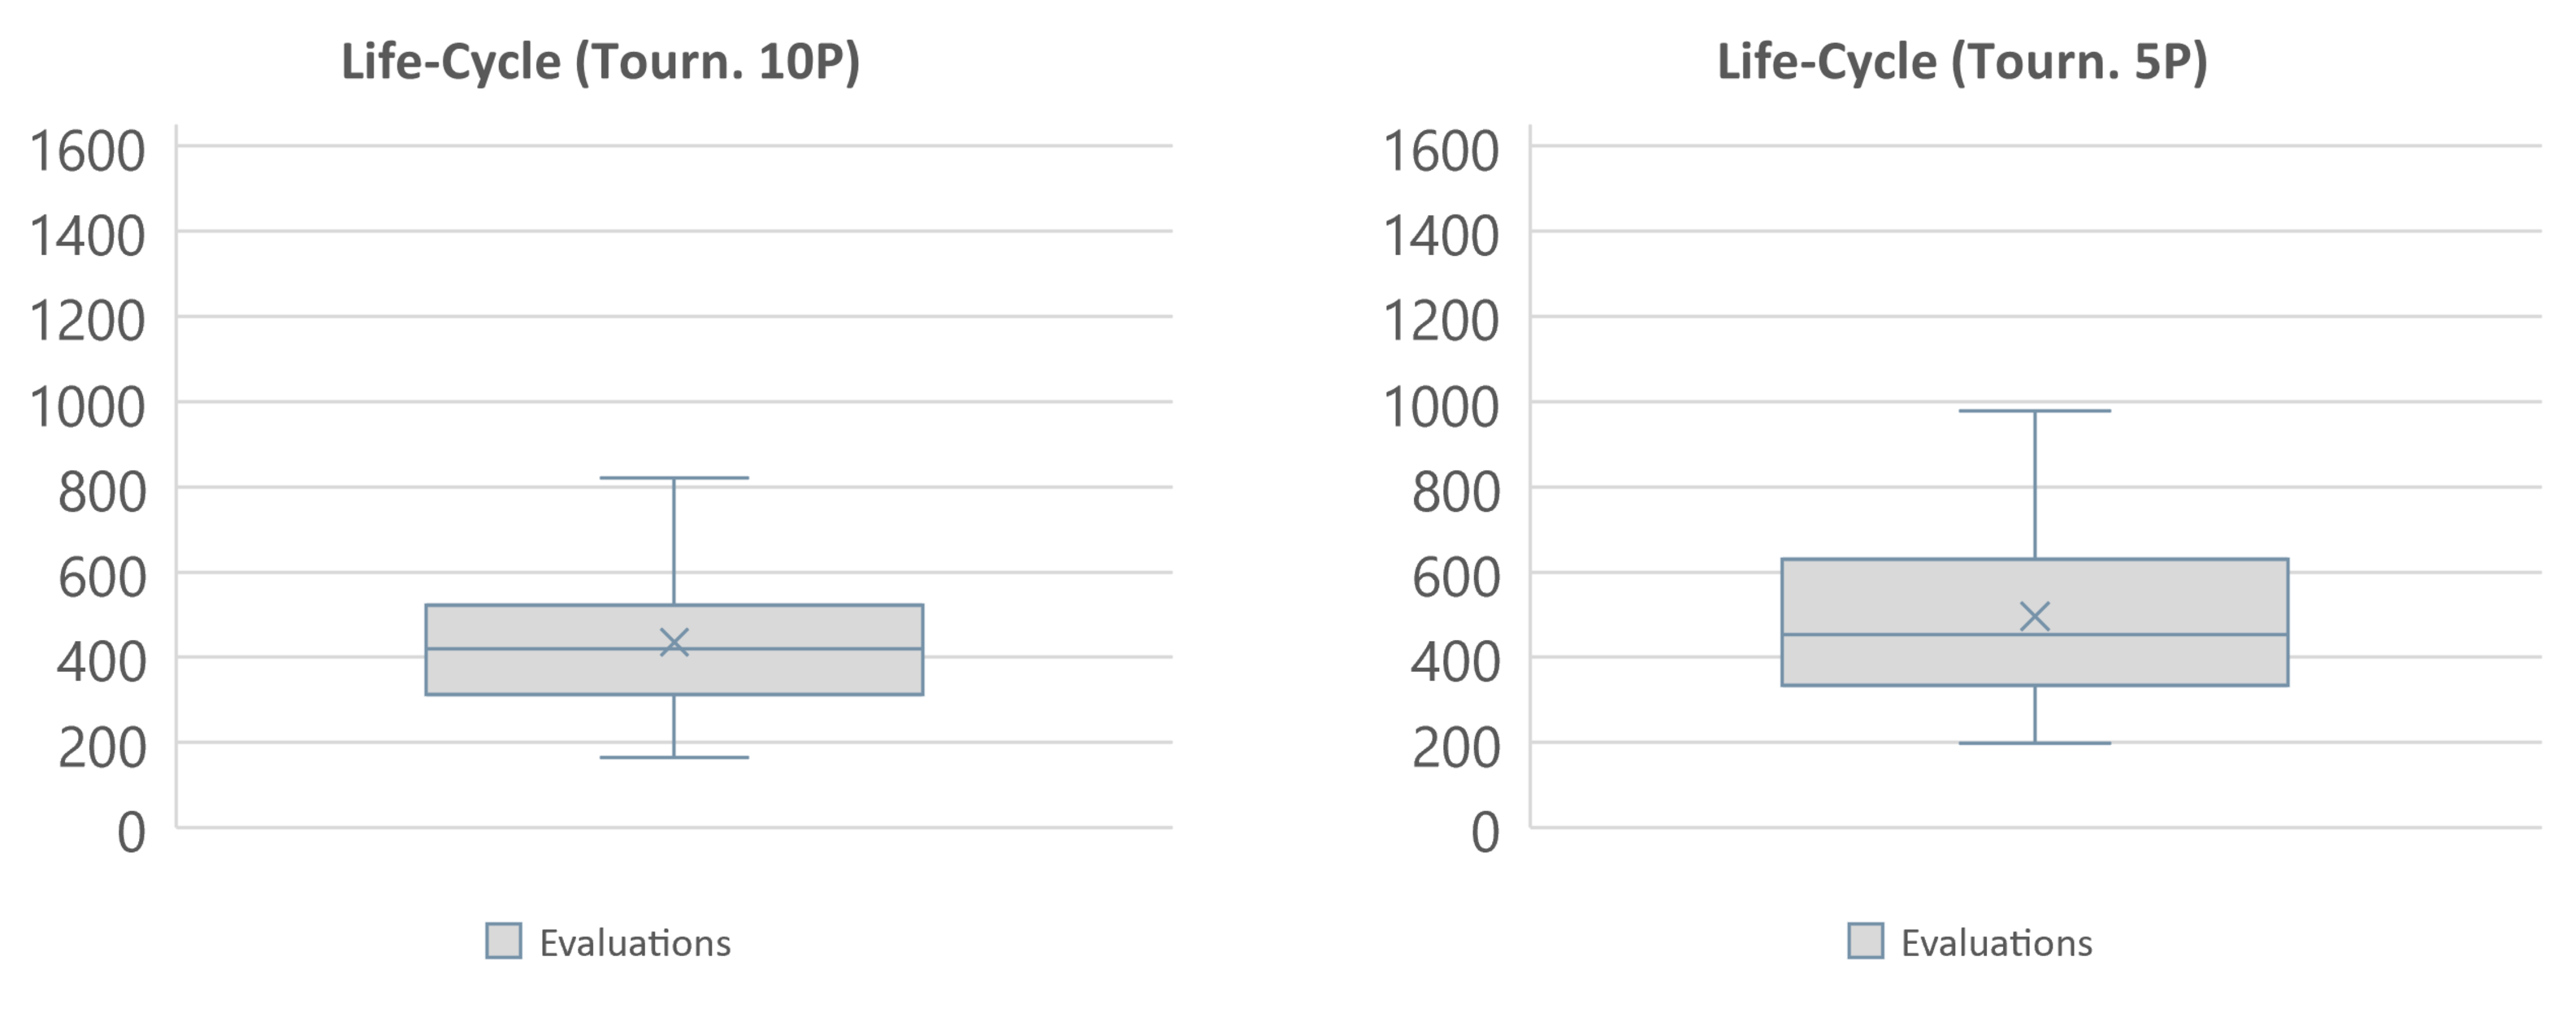
\includegraphics[width=\textwidth]{img/fig7_experiment02_chart.pdf}}
    \caption{Box and Whisker chart for the Experiment 2: Life-Cycle Tournament selection (10 versus 5 processes).} \label{fig.experiment2}
    \end{figure}


\subsubsection{Experiment 3} The goal of our third experiment was to follow and
study the behavior of the Life-Cycle algorithm that continued converging on the
solution. For this experiment, we remained using minimal delays (thousands of a
second magnitude). For this experiment, we only used tournament selection for
the reproduction, on the first configuration running the Life-Cycle on six
processes, two of whom was the Death process, versus the second configuration
where we reduced the processes to the minimum (five) but increasing the (Death)
goal approval range to 115. We show the summarized results in
Table~\ref{tab.experiment3}, and Figure~\ref{fig.experiment3} shows their Box
and Whisker chart.

\begin{table}[]
    \centering        
    \caption{Experiment 3 results, Life-Cycle Tournament: 6 processes (Death x2) versus 5 processes (80 to 115 goal).}\label{tab.experiment3}
    \begin{tabular}{|l|l|l|l|l|l|l|l|l|}
    \hline
    Run & \multicolumn{4}{l|}{LifeCycle (Tourn. 6P, Death x2)} & \multicolumn{4}{l|}{LifeCycle (Tourn. 5P, 80-115g)} \\ \hline
    1-60 & Last Gen. & Eval. & Time (sec) & Eval/sec & Last Gen. & Eval. & Time (sec) & Eval/sec \\ \hline
    Avg. & 8.0 & 483 & 0.846 & 571 & 6.4 & 384 & 0.695 & 553 \\ \hline
    \end{tabular}
    \end{table}

\begin{figure}
    \fbox{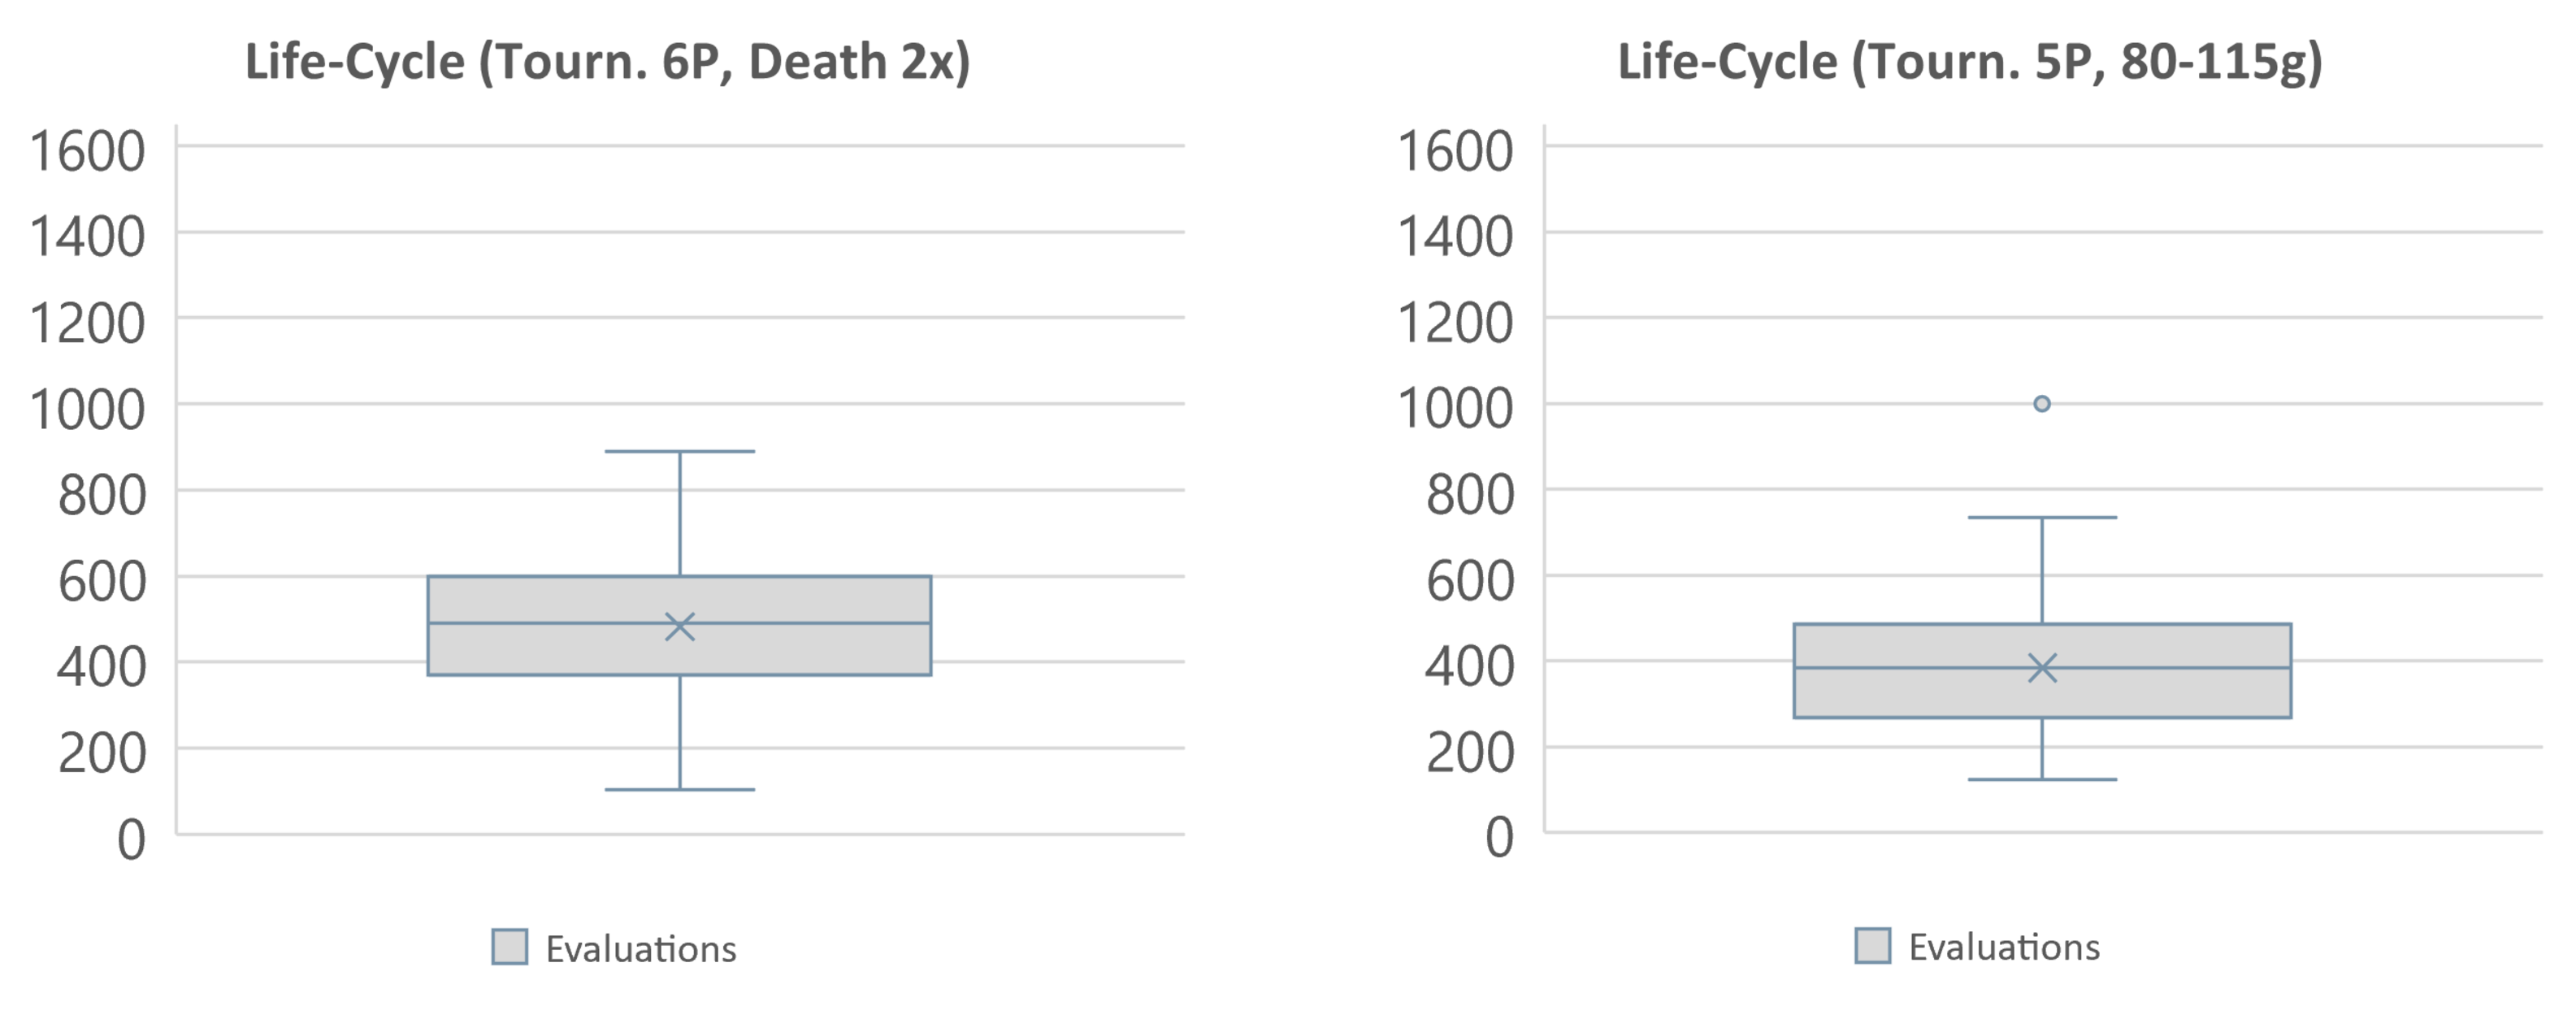
\includegraphics[width=\textwidth]{img/fig8_experiment03_chart.pdf}}
    \caption{Box and Whisker chart for the Experiment 3: Life-Cycle Tournament (6 processes double Death, versus 5 processes with an 80 to 115 goal approval).} \label{fig.experiment3}
    \end{figure}


\subsubsection{Experiment 4} The goal of our fourth and last experiment was to
follow and study the behavior of the Life-Cycle algorithm that continued
converging on the solution. For this experiment, we remained using minimal
delays (thousands of a second magnitude). For this experiment, we compared the
OneMax DEAP implementation versus the Life-Cycle algorithm, only using
tournament selection for the reproduction, with the Life-Cycle configuration
running on the minimum (five) processes but increasing the (Death) goal
approval range to 125. We show the summarized results in
Table~\ref{tab.experiment4}, and Figure~\ref{fig.experiment4} shows their Box
and Whisker chart.

\begin{table}[]
    \centering        
    \caption{Experiment 4 results, OneMax DEAP versus Life-Cycle Tournament: 5 processes (80 to 125 goal).}\label{tab.experiment4}
    \begin{tabular}{|l|l|l|l|l|l|l|l|l|}
    \hline
    Run & \multicolumn{4}{l|}{OneMax DEAP} & \multicolumn{4}{l|}{Life-Cycle (Tourn. 5P, 80-125g)} \\ \hline
    1-60 & Last Gen. & Eval. & Time (sec) & Eval/sec & Last Gen. & Eval. & Time (sec) & Eval/sec \\ \hline
    Avg. & 6.5 & 391 & 0.036 & 10,836 & 6.3 & 377 & 0.678 & 556 \\ \hline
    \end{tabular}
    \end{table}

\begin{figure}
    \fbox{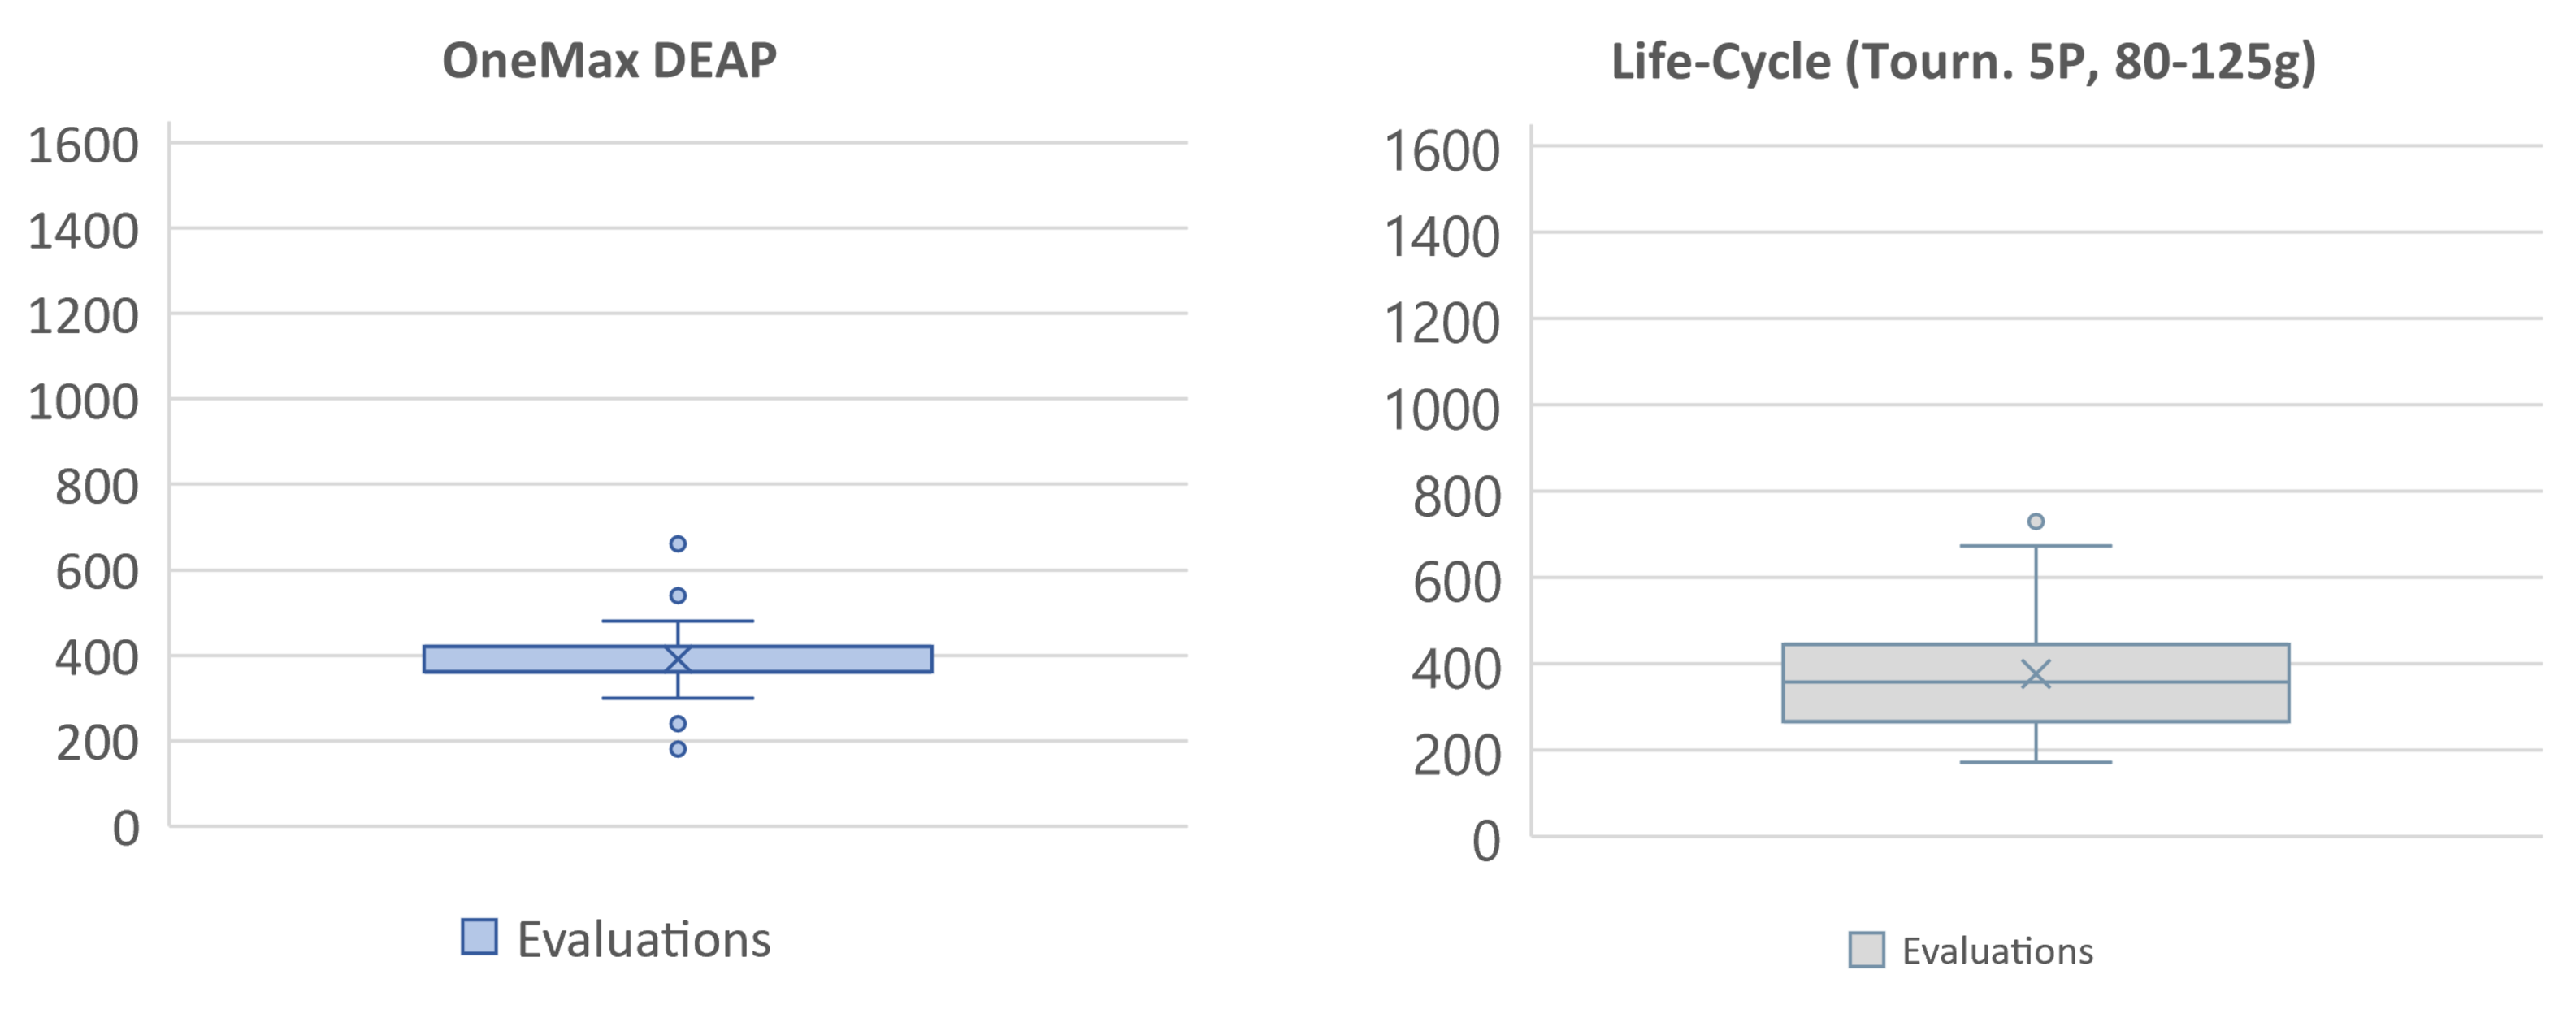
\includegraphics[width=\textwidth]{img/fig9_experiment4_chart.pdf}}
    \caption{Box and Whisker chart for the Experiment 4: OneMax DEAP versus Life-Cycle Tournament (5 processes with an 80 to 125 goal approval).} \label{fig.experiment4}
    \end{figure}


\section{Discussion}
\label{section.discussion}

At some crucial moments during our research, we got the feeling we were doing
nature reverse engineering. One strategy was to let our imagination run wild
and go for the simple solution. One of our earlier experiment's findings was to
find balance, like the yin and yang, between death and reproduction.

In our experiments, we found that when solving simple problems, the cost of
communication between containers can become a factor to increase the total
performance time, even though, we believe that the opposite must also be true.
When solving complex problems, distributing the work on multiple resources
should reduce throughput time, making the communication cost negligible.

We must acknowledge the performance time of the DEAP library
\cite{fortin2012deap} is highly efficient and short, due in part because the
processing work execution is on a single processor with multiple cores, where
the communication time is nearly non-existent. In contrast, our algorithm
implementation requires a minimum of five containers and a message queue
server. Even though the container work has proven to be very effective and
efficient \cite{merelo2016performance,valdez2021container}, we must consider
some time was added to our experiments by the minimal delays (in the thousands
of a second magnitude) we used to keep the process execution relatively random,
to mimic how the life-cycle stages work in nature \cite{read1968system}. As
future work, we could test the Life-Cycle algorithm behavior by eliminating all
remaining delays.

This scheme allows for multiple parameter's fine tuning, granting us the
freedom to experiment with different selection and reproduction strategies
simultaneously, which will impact how fast it finds the solution and the
obtained quality.


\section{Conclusions}
\label{section.conclusions}

We implemented the algorithm with Docker containers by solving the OneMax
problem comparing it with a traditional (sequential) GA algorithm, where it
showed favorable and promising results. To further validate this work, we could
use control or some more complex and demanding problem that requires computing
real numbers \cite{stanley2002evolving,miikkulainen2019evolving}.

As the complexity of problems increases, it is essential to have a scalable,
replicable, and fault-tolerant model that uses collaborative techniques to work
in the cloud, where multiple resources will be communicating asynchronously.
This research has shown that it is possible to evolve a population of
individuals, similar to a Genetic Algorithm (GA), using a distributed,
parallel, and asynchronous methodology.

\begin{acknowledgement}
    This paper has been supported in part by projects DeepBio (TIN2017--85727--C4--2--P) and TecNM Project 11356.21\@.
\end{acknowledgement}

% ---- Bibliography ----
% BibTeX users should specify bibliography style 'splncs04'.
% References will then be sorted and formatted in the correct style.
%
\bibliographystyle{splncs04}
\bibliography{bib/bibliografia.bib}

\end{document}
